\documentclass[format=acmsmall, review=false]{acmart}
\usepackage{tikz}
\usetikzlibrary{patterns,patterns.meta}
\usetikzlibrary{arrows.meta}

\begin{document}

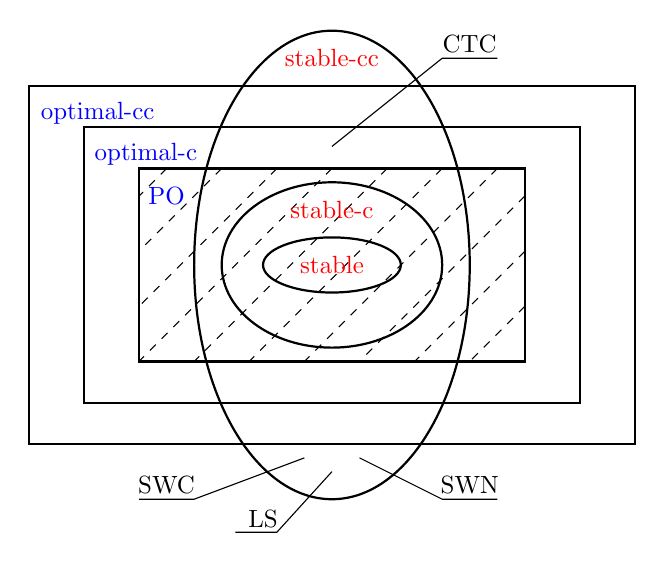
\begin{tikzpicture}[scale=0.35, sibling distance=5em,
  every node/.style = {scale=0.9, shape=circle, draw=none, align=center},
    outline/.style={draw=#1,thick,fill=#1!100}]
  every draw/.style = {scale=1}
  \draw[color=black,thick] (-1,2) rectangle (21,15);
  \draw[color=black,thick] (1,3.5) rectangle (19,13.5);
  \draw[draw=black, thick] (3,5) rectangle (17,12);
  \draw[dashed,color=black] (4,12) -- (3,11);
  \draw[dashed,color=black] (6,12) -- (3,9);
  \draw[dashed,color=black] (8,12) -- (3,7);
  \draw[dashed,color=black] (10,12) -- (3,5);
  \draw[dashed,color=black] (12,12) -- (5,5);
  \draw[dashed,color=black] (14,12) -- (7,5);
  \draw[dashed,color=black] (16,12) -- (9,5);
  \draw[dashed,color=black] (17,11) -- (11,5);
  \draw[dashed,color=black] (17,9) -- (13,5);
  \draw[dashed,color=black] (17,7) -- (15,5);
 
  \draw[color=black,thick] (10,8.5) ellipse (2.5 and 1);
  \draw[color=black,thick] (10,8.5) ellipse (4 and 3);
  \draw[color=black,thick] (10,8.5) ellipse (5 and 8.5);
  
  \node[color=blue] (node1) at (1.5,14) {optimal-cc};
  \node[color=blue] (node2) at (3.25,12.5) {optimal-c};
  \node[color=blue] (node3) at (4,11) {PO};
  \node[color=red] (node4) at (10,8.5) {stable};
  \node[color=red] (node5) at (10,10.5) {stable-c};
  \node[rectangle,color=red] (node6) at (10,16) {stable-cc};
  
  
  
  \draw[color=black] (9,1.5) -- (5,0) -- (3,0);
  \draw[color=black] (10,1) -- (8,-1.2) -- (6.5,-1.2);
  \draw[color=black] (11,1.5) -- (14,0) -- (16,0);
  \draw[color=black] (10,12.8) -- (14,16) -- (16,16);
  \node[rectangle,color=black] (node7) at (15,16.5) {CTC};
  \node[rectangle,color=black] (node8) at (4,0.5) {SWC};
  \node[rectangle,color=black] (node9) at (7.5,-0.7) {LS};
  \node[rectangle,color=black] (node10) at (15,0.5) {SWN};
  
\end{tikzpicture}

\end{document}